
\documentclass[conference]{IEEEtran}

\usepackage{url}
\usepackage{verbatim}
\usepackage{multirow}
\usepackage{float}

%\usepackage{caption}

\usepackage{algorithm}
\usepackage{todonotes}
\usepackage{graphicx}

\usepackage{ifpdf}
\ifpdf
\usepackage{epstopdf}
\fi
\usepackage{booktabs}
\usepackage{multirow}
\usepackage{siunitx}
\usepackage{array,tikz}
\usepackage{soul}

\usetikzlibrary{tikzmark,arrows.meta}
% Spectra template example
\newcolumntype{M}{>{\centering\mbox{}\vfill\arraybackslash}m{50pt}<{\vfill}}

\usepackage{array}% http://ctan.org/pkg/array

\usepackage{amsmath}
\newcommand\norm[1]{\left\lVert#1\right\rVert}
%\usepackage{cleveref}

% correct bad hyphenation here
\hyphenation{op-tical net-works semi-conduc-tor}

\newcommand{\specialcell}[2][l]{%
  \begin{tabular}[#1]{@{}l@{}}#2\end{tabular}}
 
% Equation Numbers
%\renewcommand{\theequation}{\arabic{section}.\arabic{equation}}
\usepackage{chngcntr}

\usepackage{color}
\DeclareRobustCommand{\hlcyan}[1]{{\sethlcolor{cyan}\hl{#1}}}
\DeclareRobustCommand{\hlorange}[1]{{\sethlcolor{orange}\hl{#1}}}
%\counterwithin*{equation}{section}

\newcommand{\NA}{---}

\begin{document}
%\onecolumn
%
% paper title
\title{Classification of Stars using Stellar Spectra collected by the Sloan Digital Sky Survey}

\author{\IEEEauthorblockN{Michael Brice}
\IEEEauthorblockA{\textit{Computer Science Department} \\
\textit{Central Washington University}\\
Ellensburg, WA, USA \\ michael.brice@cwu.edu}
\and
\IEEEauthorblockN{ R\u azvan Andonie}
\IEEEauthorblockA{\textit{Computer Science Department} \\
\textit{Central Washington University}\\
Ellensburg, WA, USA\\
andonie@cwu.edu}
}
%\author{
%\IEEEauthorblockN{Michael Brice\IEEEauthorrefmark{1}}
%\IEEEauthorblockN{R\u azvan Andonie\IEEEauthorrefmark{1} }

%\IEEEauthorblockA{\IEEEauthorrefmark{1}Computer Science Department, Central Washington University, Ellensburg, USA }
%}

\maketitle

% ============================================================================================================
\begin{abstract}
The classification of stellar spectra is a fundamental task in stellar astrophysics. There have been many explorations into the
automated classification of stellar spectra but few that involve the Sloan Digital Sky Survey (SDSS). We use the SDSS dataset since it is the most important stellar spectra database available today. In our approach, we apply redshift corrections to the
spectra and reduce the number of flux measurements by feature selection. Then we apply standard classifier methods: Random
Forest and Support Vector Machine. We compare the accuracy of feature selection and classifier combinations
for redshifted stellar spectra and rest stellar spectra. Even though redshifted stellar spectra create feature matrix discrepancies,
classifiers utilizing redshifted stellar spectra perform with high accuracy. This creates a viable option for automated classification
of stellar spectra without having to identify the redshift value.
\end{abstract}

% ============================================================================================================
\IEEEpeerreviewmaketitle
\begin{IEEEkeywords} 
Stellar Spectra Classification, Redshift, Feature Selection, Random Forest, Support Vector Machine, Chi Squared, Fisher, Imbalanced Data,  Sloan Digital Sky Survey
\end{IEEEkeywords} 

\todo[inline, color = green!35]{REVIEW NO. 1

Comments to the authors:
    There are two major critical comments for this paper:
    
1. The purpose of classification of stars is not clearly explained, and 
    appropriate machine learning formalization is missing. That is, why 
    classification was used, how many output classes, how many samples per class, 
    what are misclassification costs? - all these choices need to be justified by 
    application requirements (and this is completely missing)
    
2. It is not clear whether the paper aims at descriptive data-analytic 
    modeling or predictive one. If the goal is prediction, then the paper should 
    explain what is the test set and how each method's complexity parameters were 
    tuned (this is completely missing from the presentation)}

\todo[inline, color = red!65]{If it is highlighted in blue it is referencing comment 1. If it is highlighted in orange it is referencing comment 2.}
% ============================================================================================================
\section{Introduction}\label{sec:intro}

Stellar classification is a fundamental task in stellar astrophysics. Traditionally, stellar spectra are classified using statistical
tests. Stellar spectra are either classified by determining the wavelengths of emission and absorption lines using wavelet
transformations, statistical analysis, and using references to the Harvard spectral classification system or they are classified
by comparing the approximate curve of the spectra to that of templates using statistical tests. The traditional classification
schemes require complex data transformations and analysis to identify the class of a star based on its spectrum.

Presently, the Sloan Digital Sky Survey (SDSS) is creating the most detailed three-dimensional maps of the Universe ever
made, with deep multi-color images of one-third of the sky, and spectra for more than three million astronomical objects \cite{sdss}. The SDSS provides stellar spectra with redshift wavelengths.  In our work, we will use the SDSS data run 14 optical spectra dataset for stars, the most important stellar spectra database available today. So far, there are only a few classification results reported for this database.

In previous work related to machine learning classification of stellar spectra, Xing and Guo \cite{Xing}, Zhang \textit{et al.} \cite{Luo}, and Yi and Pan \cite{YI} used stellar spectra sources such as Pickles \cite{Pickles} and Jacoby \cite{Jacoby}. Bazarghan and Gupta \cite{Bazarghan} also used the stellar spectra sources Jacoby and SDSS \cite{York}. 

Xing and Guo \cite{Xing} used Principle Component Analysis (PCA) and wavelet reduction to reduce the large number of flux measurements, which for SDSS range from 3,800 to 4,000 measurements. We have to note that they reduced the number of flux measurements without using  machine learning feature selection or extraction methods. Zhang \textit{et al.} \cite{Luo} pre-processed the data by filtering out the high frequency components of stellar spectra using continuum normalization and did not reduce the number of features.  

Recently, Pasquet-Itam \textit{et al.} applied several methods to classify quasars in the SDSS Stripe 82 and also to predict the photometric redshifts of quasars \cite{Pasquet2018}. SDSS Stripe 82 is a different SDSS dataset than data run 14 optical spectra for stars. It is important to note that a quasar is an extremely luminous galactic nuclei, fundamentally different from a star. 

Pasquet-Itam \textit{et al.} used Convolutional Neural Network (CNN), K-nearest neighbors (KNN), Support Vector Machine (SVM), Random Forest (RF), and a Gaussian Process classifier. The input for the CNN were Light Curve Images which are built from light curves of each object in the five ugriz filters, so as to include both the crucial information of the variability and the colors in the learning of the network. The \textit{ugriz filters} are u (Ultraviolet), g (Green), r (Red), i (Near Infrared), z (Infrared). Theses filters are like a filter on a camera and it only lets certain wavelengths through, which is not data filtering. A \textit{light curve} is the apparent, or differential, brightness or magnitude taken over multiple nights \cite{Chromey}. For SDSS Stripe 82, the maximum number of nights of observation is 3,340 nights \cite{Pasquet2018}. Our results do not compare to the results found in \cite{Pasquet2018} because our data is significantly different:  Pasquet-Itam \textit{et al.} utilize light curve images where we utilize spectra. 

The amount of astronomical data increases exponentially, and the complexity and dimension of astronomical data are also
growing rapidly. The SDSS is a representative example. Extracting information from such data becomes a challenging problem.
For example, some classification algorithms can only be employed in the low-dimensional spaces, so feature selection and
feature extraction become important topics. A review of feature selection methods for high dimensional data in astronomy can
be found in \cite{Zheng}.

Our contribution is a novel approach to stellar classification. In contrast to previous approaches, our method is characterized by the following:

\begin{itemize}
	\item We avoid complex transformation and statistical analysis of the spectra space.
	\item We use spectra without redshift corrections.
	\item We use feature selection to reduce the number of flux measurements. Feature selection may destroy the shape and the structure of each stellar spectrum by only using the most relevant flux measurements. This is in contrast to \cite{Xing}, where PCA and wavelet reduction are used to reduce the number of flux measurements while maintaining the shape and structure of each spectra. 
\end{itemize}

For the SDSS spectra, we obtained the best results using the Fisher feature selection and the RF classifier. Our method can be used to classify stars using redshifted stellar spectra (e.g. stellar spectra that has not been redshift corrected). Our experimental results outperform the ones reported in \cite{Xing}, where wavelet reduction and SVMs were used for SDSS spectra.

The structure of the paper is as follows. Section \ref{sec:astro} provides relevant astronomy background. Section \ref{sec:approach} introduces our approach to stellar classification. In Section \ref{sec:experiments} the experimental setup and results are explained. Section \ref{sec:conclusion} presents our conclusions.

% ============================================================================================================
\section{Astronomy Background}\label{sec:astro}

	We start by introducing some basic definitions related to astronomy. Details may be found in standard sources like \cite{Carroll} and \cite{Chromey}. 

% ============================================================================================================
	\subsection{Stellar Spectra} \label{sec:spectra}

        The \textit{spectra} are  defined as the way in which light is distributed with wavelength \cite{Chromey}. Incandescent light bulbs, when viewed with the unaided eye, emit white light, but when viewed through a prism or a diffraction grating, the bulb appears to be emitting a rainbow or spectrum of light. Stellar spectra work the same way. Stellar spectra are collected by a spectrograph, which utilizes a fine tuned diffraction grating to collect the spectrum of a star. Unlike the example with the incandescent light bulb, stellar spectra have interesting properties. 

        The stellar spectra from the SDSS dataset contain wavelength measurements and flux measurements. The \textit{wavelengths} are discrete values that represent a range of wavelengths of light. For example, a wavelength value can be 6,000$\pm5$ $\mathring{A}ngstr\ddot{o}ms$ ($\mathring{A}$). \textit{Flux measurements} are the number of photons that pass through an area per second per measured wavelength. The shape and features of stellar spectra are defined by the flux measurements at particular wavelength values. Fig. \ref{fig:G2} shows an example spectrum of a flux scaled G2 (Sun like) star. The downward spikes seen in Fig. \ref{fig:G2} are absorption lines.

	Absorption lines are one of the many interesting properties found in stellar spectra. Absorption lines indicate the types of elements present in a star such as hydrogen, helium, and heavy metals and are key to classifying stars.
        
        % G2 Spectra Plot
        \begin{figure}
            \centering
            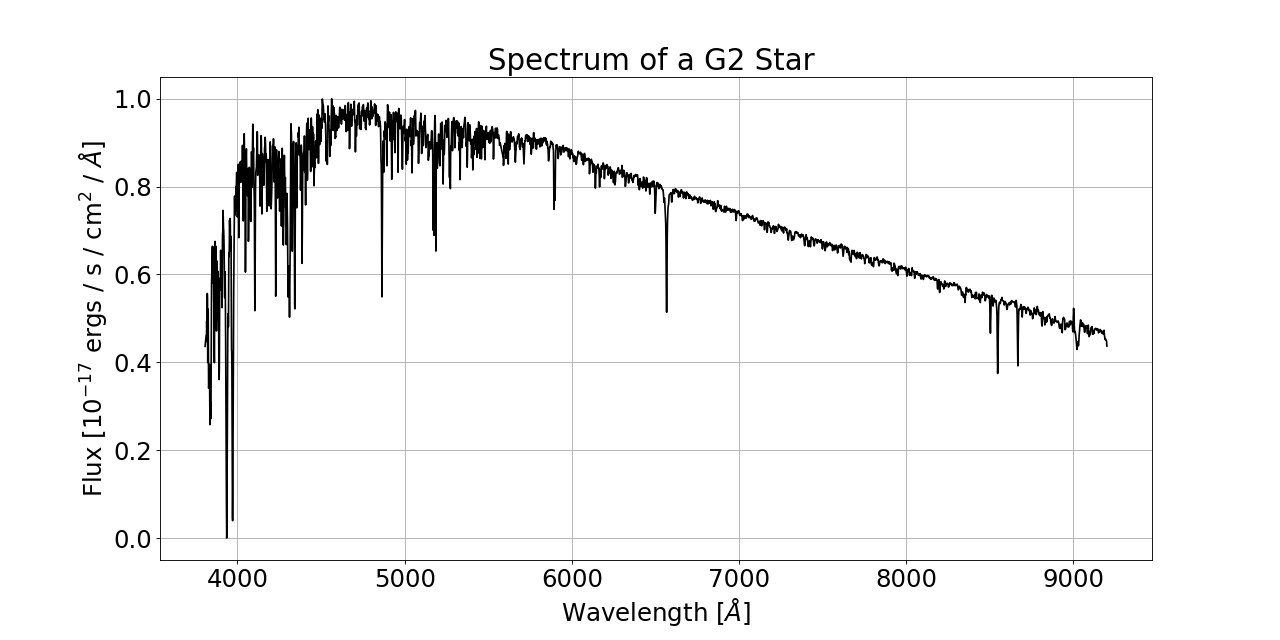
\includegraphics[width=3.5in]{G2.png}
            \caption{Example: Stellar Spectrum of a flux scaled G2 star collected by the SDSS.}
            \label{fig:G2}
        \end{figure}

% ============================================================================================================
	\subsection{Stellar Classification Types}\label{sec:classes}

	There are two types of stellar classification schemes: The Harvard spectral classification and the Morgan - Keenan Luminosity Classes (M-K) \cite{Carroll}. The Harvard spectral classification is a surface temperature classification that uses the spectra from stars to categorize into groups labeled O, B, A, F, G, K, and M. These groups are then divided into 0 - 9. For example, A0 - A9 where A0 is an early A type star and A9 as a late A star \cite{Carroll}. The Harvard spectral classification is a one dimensional system that utilizes absorption lines to characterize stellar types. The M-K Classes extends on the Harvard spectral classification by adding the luminosity of the star. The M-K adds the identifiers of I to VI for Super Giants, Bright Giants, Giants, Sub-Giants, Main Sequence (Dwarfs), and Sub-Dwarfs \cite{Carroll}. For example, Betelgeuse is a red super giant and a stellar class of M1 (Harvard) Ia (M-K) star and Proxima Centauri is a main sequence red dwarf and a stellar class of M6 V star. 
        
        The data provided by the SDSS has the Harvard spectral classes of the spectra and not the M-K luminosity classes. This paper is only concerned with the Harvard spectral classification.

% ============================================================================================================	        
	\subsection{Importance of Stellar Classes}\label{sec:importance}

        	Astronomers use stellar classes, in conjunction with other data, to learn many details about stars. The Hertzsprung-Russell (H-R) diagram, shown in Fig. \ref{fig:HR}, is a plot of stars where the horizontal axis is the spectral class or surface temperature and the vertical axis is the luminosity or absolute magnitude.
  
        % Hertzsprung Russel Diagram figure || This image can be removed if page space is needed
        \begin{figure}
            \centering
            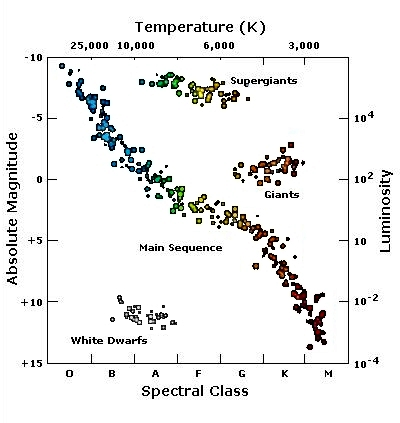
\includegraphics[scale = .37]{HR.jpg} %51
            \caption{Hertzsprung Russell Diagram \cite{hr}}
            \label{fig:HR}
        \end{figure}

        The location of a star on the H-R diagram tells astronomers information about that star. For example, stellar evolution can be mapped out on the H-R diagram \cite{Carroll}. The location of a star on the H-R diagram defines whether it is in the main sequence, a giant, a super giant, or whether the star has stopped fusion of Hydrogen and is fusing Helium, or if it has stopped fusing Helium and so on \cite{Carroll}.

% ============================================================================================================		
	\subsection{Redshift}\label{sec:redshift}

	\textit{Redshift} is caused by the relative motion of a star with respect to an observer through the Doppler effect on light. When a star moves away from an observer, the wavelengths of light appear to be longer, or, in terms of the visible spectrum, redder. Redshift causes the flux measurements to be shifted compared to what would have been observed at rest \cite{Carroll, Chromey}.

All stars have different redshift values. Redshift is defined by (\ref{eq:red}), where \textit{Z} is the redshift value and $\lambda$ is the wavelength \cite{Carroll, Chromey}. Equation (\ref{eq:flux1})  defines how the flux density changes due to redshift, where \textit{f} is the flux density at wavelength $\lambda$ (see \cite{Chromey}). However, for the purpose of this paper, since \textit{Z} for stars from the SDSS database have \textit{Z} $\ll$ 1, (\ref{eq:flux2}) is used: 
        
        % Redshift equation
        \begin{equation}\label{eq:red}
            Z = \frac{\lambda_{observed} - \lambda_{rest}}{\lambda_{rest}}
        \end{equation}

	% Flux Redshift equation
        \begin{equation}\label{eq:flux1}
            f(\lambda_{rest}) = (1 + Z)^2 f(\lambda_{observed}) 
        \end{equation}

	% Flux Redshift equation
        \begin{equation}\label{eq:flux2}
            f(\lambda_{rest}) \approx f(\lambda_{observed})
        \end{equation}


 Fig. \ref{fig:redshift} shows an example of redshift. Notice that the two spectra are identical, but shifted. The dashed line represents spectra with redshift and the solid line represents the same spectra but with redshift corrections applied. Redshift correction shifts the wavelengths from their observed values to the values that would have been observed if the star was at rest relative to the observer, which is referred to as \textit{rest wavelengths} in this paper. 

	% Visual of Redshift
        \begin{figure}
            \centering
            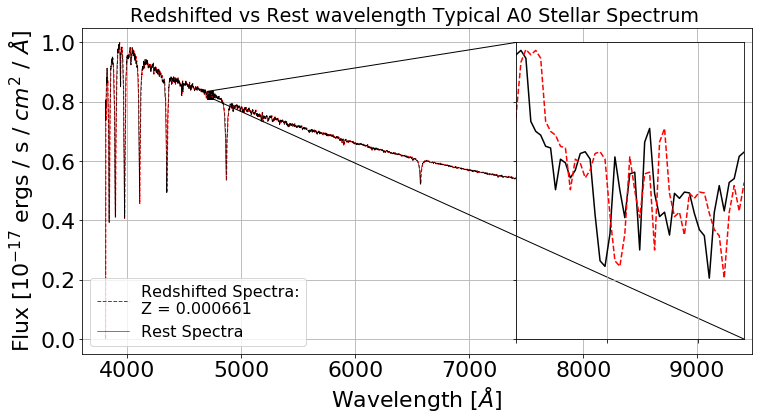
\includegraphics[width=3.5in]{redshift.png}
            \caption{Example of redshift}
            \label{fig:redshift}
        \end{figure}

% ============================================================================================================
\section{Our approach}\label{sec:approach}

\hlorange{Our goal is to classify stars from the SDSS database based on stellar spectra}. \todo[inline, color = red!65]{Maybe we could write "Our goal is to predict star classes from the SDSS database based on stellar spectra." ?}In this section, we describe the data, the pre-processing steps, and the feature selection and classification techniques for stellar classification. 
		
% ============================================================================================================	
	\subsection{Data}\label{sec:data}

	The stellar spectra collected by the SDSS are pre-processed by SDSS scientists through the methods presented by Dawson \textit{et al. }\cite{Dawson} and Stoughton \textit{et al.}  \cite{Stoughton}. There are two spectrographs used by the SDSS to collect the stellar spectra: the Baryon Oscillation Spectroscopic Survey (BOSS) spectrograph and the SDSS spectrograph. The data used in this paper was collected using the SDSS spectrograph. The SDSS spectrograph is identical to the BOSS spectrograph except the BOSS spectrograph has upgraded Charged Coupled Device (CCD) cameras, a larger wavelength sensitivity, and a larger number of astronomical objects that can be simultaneously observed \cite{boss}. Therefore, due to the limited literature of the SDSS spectrograph, the more in depth descriptions of the BOSS spectrograph will suffice and are presented by Smee \textit{et al.} \cite{Smee}.  

	The dataset used in this paper comes from SDSS data run 14, which collected 600,967 stellar spectra. Some of the stellar spectra were rejected from this study because they were not able to be classified (e.g. the documented stellar class is not O, B, A, F, G, K, and M with sub-classes of 0 - 9). Other spectra were rejected because large portions of flux measurements were missing due to CCD or other instrument failures. Stellar spectra with more than half of their spectrum missing were also rejected. The usable dataset contains 578,346 stellar spectra and 22 of the 70 classes. These spectra are used as the input vectors, with each spectrum having 3,800 to 4,000 features. These features are the flux measurements. \hlcyan{The distribution of the classes from this dataset is highly imbalanced, as seen in Fig.} \ref{fig:dist}. We balanced the dataset using: \textit{i)} undersampling (removing samples); and \textit{ii)}  hybrid sampling, consisting in both undersampling and oversampling (duplicating samples)  \cite{Japkowicz}. \hlcyan{Undersampling results in each class having 572 samples} for a total of 12,584 samples. \hlcyan{Hybrid sampling results in each class having 16,682 samples} for a total of 367,004 samples. \hlcyan{Data balancing and Data pre-processing (Section} \ref{sec:pre-proc}) \hlcyan{do not change the output classes found in Fig.} \ref{fig:dist}. \todo[inline, color = red!65]{I added this sentence}

       % Distribution of classes in dataset
        \begin{figure}
            \centering
            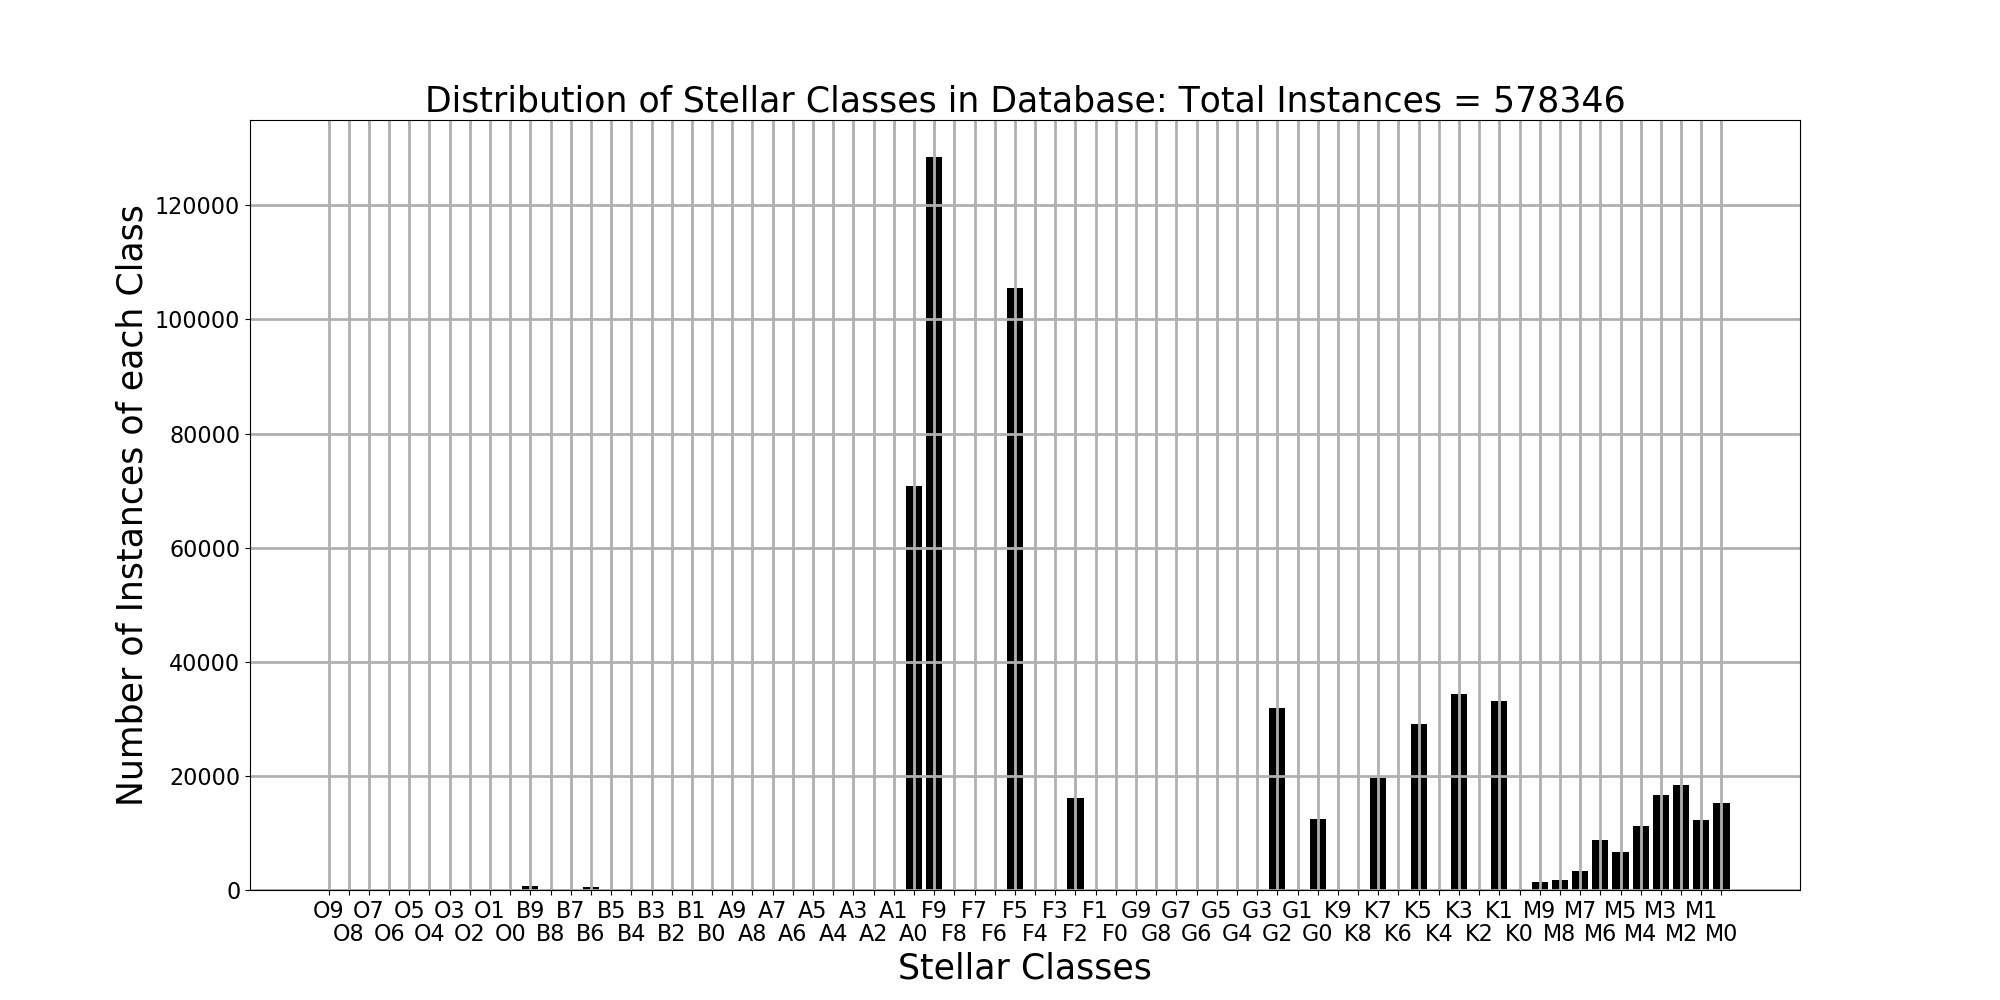
\includegraphics[width=3.5in]{Distribution.png}
            \caption{\hlcyan{Distribution of classes in the dataset}}
            \label{fig:dist}
        \end{figure}


% ============================================================================================================
	\subsection{Data pre-processing}\label{sec:pre-proc}

The flux intensity for a given class of star varies for a variety of reasons, including proximity to the spectrograph and the star's luminosity. To resolve this issue, the flux is scaled from 0 to 1 using \eqref{eq:scale}, where $f_i$ is the \(i\)th  flux measurement, $f_{max}$ and $f_{min}$ are the maximum and minimum flux measurements respectively, and $f_{i, scaled}$ is the resulting scaled flux:
        
        % Flux scaling equation
        \begin{equation}\label{eq:scale}
            f_{i, scaled} = \frac{f_i - f_{min}}{f_{max} - f_{min}}
        \end{equation}
        
	Each stellar spectrum in the dataset collected different amounts of flux measurements. This creates a problem when building the feature matrix, which will be described in Section \ref{sec:feature}. To overcome this problem, an average number of flux measurements is computed using the first 5,000 spectra. This average is then used to fit each spectrum to a standardized number of flux measurements. The resulting average number of flux measurements is 3,834.
        
	The next pre-processing phase deals with redshift. The data presented by the SDSS is redshifted. Due to the dataset being redshifted, the dataset is redshift corrected using (\ref{eq:red}) and the provided redshift for each spectrum. This way we create artificial rest spectra.

When the wavelengths are represented in logarithmic space, the difference between two adjacent wavelength values is 0.0001 (see \cite{dr14}). Therefore, the margin for each wavelength value is $\lambda\pm0.00005$. Using the wavelengths in logarithmic space, the artificially redshifted wavelengths are fitted to the nearest $\lambda$, within the margin of 0.00005.

        Building the feature matrix requires a template for wavelength values. The purpose of the template is to fit each stellar spectrum to identical wavelength values, because each stellar spectrum starts collecting flux measurements at different wavelength values \cite{dr14}. The first spectrum in the database with 3,834 flux measurements and wavelength values was chosen as the template for all spectra wavelength fitting. The wavelengths of this spectrum are then extracted into the template and used to fit each spectrum to a uniform set of wavelength values.

	The process of fitting takes the spectrum's first wavelength value and locates it in the template's wavelength array (Fig. \ref{fig:right}). For example, if the first wavelength value (index 0) in the spectrum's wavelength array is located at index 1 in the template's wavelength array, then the spectrum's wavelength array is "shifted" to the right. This causes index 0 of the spectrum's wavelength array to be shifted to index 1. If index 0 of the spectrum's wavelength array does not appear in the template's wavelength array, then the fitting process locates the template's index 0 in the spectrum's wavelength array (Fig. \ref{fig:left}).
        
        % Fitting wavelengths to a template examples
        \begin{figure}
            \centering
            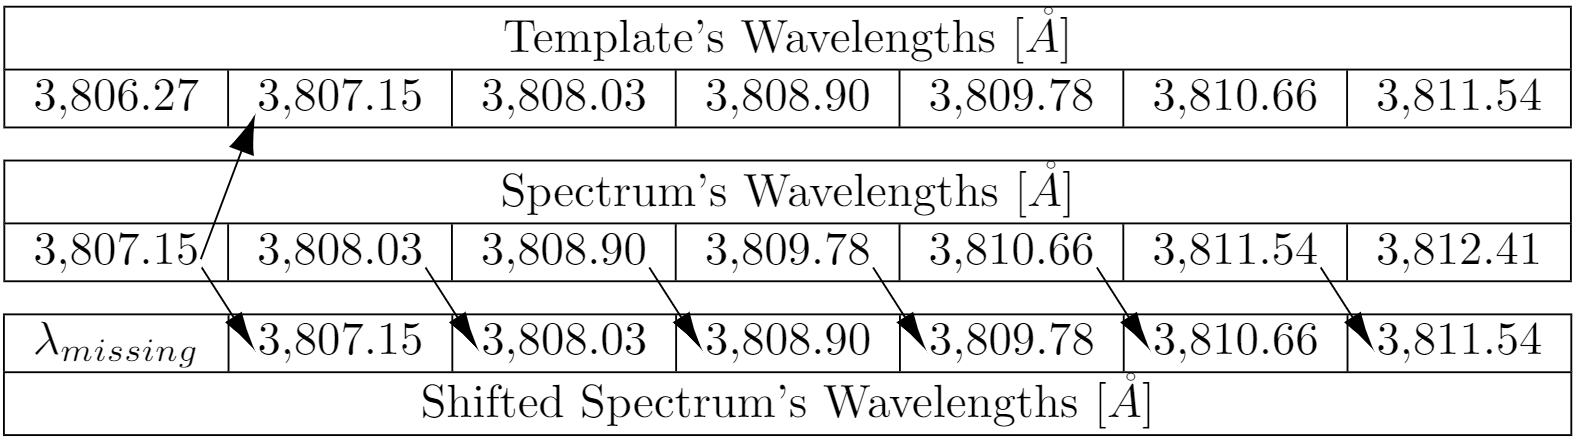
\includegraphics[width=3.5in]{figure3.png}
            \caption{Example of fitting a spectrum's wavelengths to the template wavelengths: Right Shifting.}
            \label{fig:right}
        \end{figure}

        \begin{figure}
            \centering
            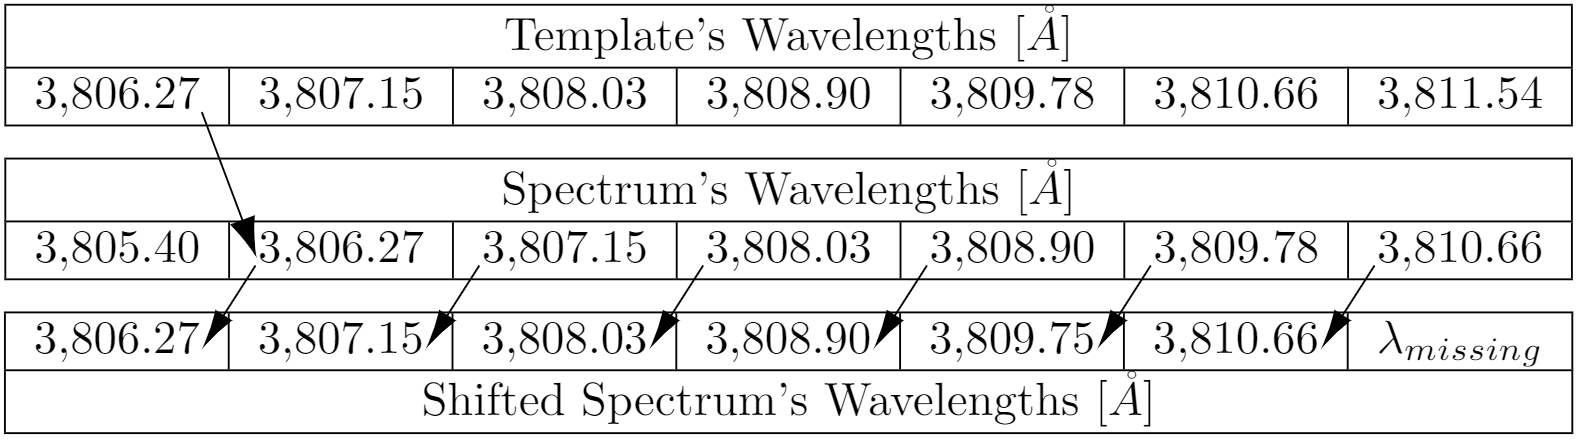
\includegraphics[width=3.5in]{figure4.png}
            \caption{Example of fitting a spectrum's wavelengths to the template wavelengths: Left Shifting.}
            \label{fig:left}
        \end{figure}

	\begin{figure}
            \centering
            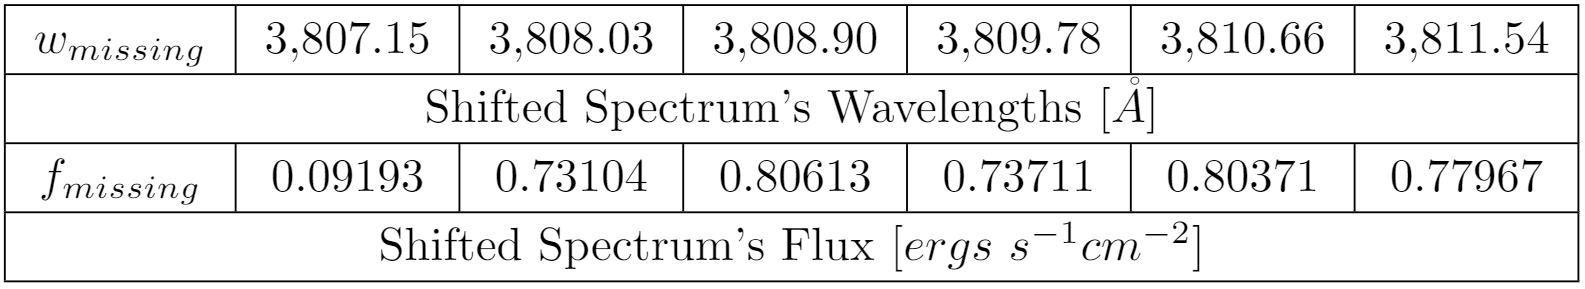
\includegraphics[width=3.5in]{figure5.png}
            \caption{Example of a spectrum's wavelengths and flux arrays after fitting to a template.}
            \label{fig:miss-f}
        \end{figure}
        
        Notice in Figs. \ref{fig:right} and \ref{fig:left} that the shifted spectrum's wavelengths appear in the same column as the template's wavelengths. The shifted spectrum's wavelength array is now fitted to the template. Since each flux measurement is directly associated with a wavelength value, the flux array is fitted in parallel to the wavelength arrays. When the wavelength array is shifted to the left or right, the flux array is shifted to the left or right by the same amount, which is apparent in Fig. \ref{fig:miss-f}.  

% ============================================================================================================
	\subsection{Feature Matrix}\label{sec:feature}

        Each stellar spectra has two arrays, a flux array that stores flux measurements and a wavelength array that stores the wavelengths that correspond to the flux measurements. The feature matrix is constructed with the rows as stellar spectra and the columns as the flux measurements that are measured at a particular wavelength (see Table \ref{tab:feature-matrix}). Specifically, the wavelength array is used as column headers in the feature matrix. 

\begin{table}
        \centering
        %\Large
        \caption{Example of the feature matrix}
        \label{tab:feature-matrix}
        \resizebox{3.5in}{!}{
        \def\arraystretch{1.2}
\begin{tabular}{|c|c|c|c|c|}
\hline
           & \begin{tabular}[c]{@{}c@{}}Wavelength:\\ 3,807.15 $\mathring{A}$\end{tabular} & \begin{tabular}[c]{@{}c@{}}Wavelength:\\ 3,808.03 $\mathring{A}$\end{tabular} & \begin{tabular}[c]{@{}c@{}}Wavelength:\\ 3,808.90 $\mathring{A}$\end{tabular} & \begin{tabular}[c]{@{}c@{}}Wavelength:\\ 3,810.66 $\mathring{A}$\end{tabular} \\ \hline
Spectrum 1 & Flux                                                     & Flux                                                      & Flux                                                       & Flux                                                       \\ \hline
Spectrum 2 & Flux                                                       & Flux                                                      & Flux                                                       & Flux                                                       \\ \hline
\end{tabular}}
\end{table}

        As stated in Section \ref{sec:pre-proc}, each stellar spectra starts at different wavelength values. To ensure that each column of the feature matrix represents flux measured at the same wavelength, each wavelength array is fitted to the wavelength array template. 

        When the wavelength array is being fitted to the wavelength template array, it can create missing values (represented by $\lambda_{missing}$), as seen in Figs. \ref{fig:right} and \ref{fig:left}. When a wavelength array is right shifted, missing values are guaranteed to form at the beginning. This is due to the first wavelength value being shifted to the right leaving no wavelength values. When a wavelength array is left shifted, a missing value forms if the last wavelength value in the spectrum is smaller than the last wavelength value in the template. After shifting the spectrum's wavelength and flux arrays, if the array length is larger than 3,834, then the spectrum's wavelength and flux arrays are cut off at index 3,833 to ensure all spectra have the same number of flux measurements.
        
        Missing wavelength values are replaced with the values from the template's wavelength array. Missing flux values (represented by $f_{missing}$) are replaced using the average of the next or last \textit{K} flux measurements. A moving average is used to ensure the continuation of the trend and that no artificial absorption lines are created. Artificial absorption lines can lead to misclassification.

% Re word this so the missing values and approximate values are more clear
        When the missing flux measurement is at the beginning of the flux array, then the next \textit{K} flux measurements are averaged using (\ref{eq:beg}), where \textit{j} is the index of $f_{missing}$ being replaced. The sequence of missing values at the beginning of the flux array is as follows: [ $\bar{f}_0$, $\bar{f}_1$, ..., $\bar{f}_w$ ], where \textit{w} is the index of the last missing value. The missing values are replaced from index \textit{w} to index 0. The computed moving average includes any estimated missing values.
        
        % Missing value approximation for missing values at the beginning of the spectra
        \begin{equation}\label{eq:beg}
            \bar{f}_j = \frac{1}{K} \sum_{i = j+1}^{K+j+1} flux_{i}
        \end{equation}
        
        When the missing flux measurement is at the end of the flux array then the last \textit{K} flux measurements are averaged using (\ref{eq:end}), where \textit{j} is the index of $f_{missing}$ being replaced and \textit{j} $>$ \textit{K}. The sequence of missing values at the end of the flux array is as follows: [ $\bar{f}_v$, $\bar{f}_{v+1}$, ..., $\bar{f}_{3,833}$ ], where \textit{v} is the index of the first missing value. The missing values are replaced starting at index \textit{v} to index 3,833. The moving average when computed includes any estimated missing values.
        
        % Missing value approximation for missing values at the end of the spectra
        \begin{equation}\label{eq:end}
            \bar{f}_j = \frac{1}{K} \sum_{i = K-j-1}^{j-1} flux_{i}
        \end{equation}
        
%        The process of fitting the spectra to a template forces the flux values to appear in the same location in the feature matrix for each stellar spectra. For example at column 0 the entire column represents flux measurements measured at the same wavelength value.
        
        A problem arises with the feature matrix because redshift causes the flux measurements to be shifted in wavelength. This causes the columns of the feature matrix to have the same flux measurement at different wavelengths for the same class. Certain flux measurements have real physical meaning such as the absorption lines. For example, the Hydrogen Alpha (H$\alpha$) absorption line is observed at rest with wavelength at 6,562.8 $\mathring{A}$ in air, but due to redshift, the H$\alpha$ line can be observed at other wavelengths such as 6,563.8 $\mathring{A}$ or 6,561.8 $\mathring{A}$. An example of how redshift changes the meaning of each column is seen in Table \ref{tab:example}. Notice how H$\alpha$ appears in different columns of the feature matrix due to redshift for the same stellar class. This is comparable to taking the pedal width of the iris dataset's \cite{Dua:2017} feature matrix and putting it in the pedal length column.  
        
        % Example of redshift in the feature matrix
        \begin{table}
        
        \centering
        %\Large
        \caption{Example of the feature matrix that has redshifted data}
        \label{tab:example}
        \resizebox{3.5in}{!}{
                \def\arraystretch{1.2}
            \begin{tabular}{|c|c|c|c|c|c|}
            \hline 
            \begin{tabular}[c]{@{}l@{}}Wavelength: \\ 6,560.8 $\mathring{A}$\end{tabular} & \begin{tabular}[c]{@{}l@{}}Wavelength: \\ 6,561.8 $\mathring{A}$\end{tabular} & \begin{tabular}[c]{@{}l@{}}Wavelength: \\ 6,562.8 $\mathring{A}$\end{tabular} & \begin{tabular}[c]{@{}l@{}}Wavelength: \\ 6,563.8 $\mathring{A}$\end{tabular} & \begin{tabular}[c]{@{}l@{}}Wavelength: \\ 6,564.8 $\mathring{A}$\end{tabular} & \begin{tabular}[c]{@{}l@{}}Star \\ Class\end{tabular} 
            \\ \hline
                & & H$\alpha$ & & & A0 \\ \hline
                & H$\alpha$ & & & & A0 \\ \hline
                & & & H$\alpha$ & & A0 \\ \hline
                & & & & H$\alpha$ & A0 \\ \hline
                H$\alpha$ & & & & & A0 \\ \hline
            \end{tabular}
        }
        \end{table}
        
	As described in Sections \ref{sec:spectra} and \ref{sec:classes}, absorption lines are a key parameter in classifying stars with the Harvard spectral classification system. The classification of a star defines the expected wavelength at which certain absorption lines occur. However, to redshift correct a spectrum, the redshift is computed using \eqref{eq:red}, where the wavelengths of known absorption lines are used.  By definition, knowing the absorption lines to perform redshift corrections also means that the class of the star is known. The other approach to determine the redshift of a spectrum utilizes statistical analysis to compare the spectra to templates, which as a by product the class of the star is known. 

	Machine learning approaches to classifying stars with redshift corrected data are redundant because the by product of redshift correcting a spectrum is the star's class.

	The redshift of stars in the SDSS dataset is small. \textit{Z} is on the order of magnitude of 0.0001. As such, absorption lines, key features of the dataset, are still grouped closely together. Classification with a large number of stellar spectra of each class with a large range of redshift values overcome the redshift problem.    

% ============================================================================================================
	\subsection{Feature selection and stellar classification}\label{sec:alg}

We used the Chi Squared \cite{scikit-learn} and Fisher \cite{reliefF} filter feature selection algorithms. For a large dataset as SDSS, the Fisher method performed best.

We used the RF and SVM classifiers, chosen because other works using these two classifiers on similar data reported good results.  For instance, Xing and Guo \cite{Xing} used a SVM to classify stellar spectra. Yi and Pan \cite{YI} applied RF to the classification of stellar spectra. 


% ============================================================================================================
\section{Experiments}\label{sec:experiments}

We performed experiments on stellar spectra from the SDSS database. In the following, we present the results of the Chi Squared and Fisher feature selection algorithm in conjunction with the RF, and SVM classifiers. The resulting best feature selection and classifier algorithm pair is then expanded on with its precision, recall, and F1 score statistics.

The results are then compared for redshifted spectra and artificial rest spectra. Artificial rest spectra are used as a baseline for comparison for the redshifted spectra. 

\hlcyan{We did not implement any misclassification costs.} \todo[inline, color = red!65]{I added this sentence}
% ============================================================================================================
	\subsection{Experimental Framework and Results}\label{sec:results}

    	The first step of the experiments is to perform data pre-processing, as described in Section \ref{sec:pre-proc}. The flux is scaled to ensure that similar classes have similar flux measurements using (\ref{eq:scale}). There are two datasets used in this paper, redshifted spectra and artificial rest spectra. Both datasets are created from the SDSS dataset. For redshifted spectra, the wavelengths are adjusted using (\ref{eq:red}) through the process described in Section \ref{sec:pre-proc}. For artificial rest spectra, this process is forgone because all of the spectra in the SDSS database is redshift corrected. The remaining parts of the data pre-processing are applied to both datasets.

	The wavelengths are fitted to a template to ensure that each spectrum's wavelength coverage is identical, which is supported by the work presented by Bazarghan and Gupta \cite{Bazarghan}. This process is described in Section \ref{sec:pre-proc}. Since each flux measurement is associated with a wavelength value when the wavelengths are fitted to the template, the flux array gets transformed identically. The process of fitting the wavelengths to the template and the flux array transformation causes missing values to appear. These missing values are approximated using a moving average, as described in Section \ref{sec:feature}, and by (\ref{eq:beg}) and (\ref{eq:end}).

%	Once the data has been pre-processed, the feature matrix is placed into a Python numpy memmap object which allows the Python implementation to access the feature matrix from a solid state drive instead of RAM. The feature matrix is roughly 18 GB in size, which is larger than the RAM on the machine used to conduct these experiments. The machine that these experiments are computed on has the following relevant specifications: AMD Ryzen 7 1800x 16 logical core CPU, 16 GB RAM, and 1 TB Samsung 860 EVO Solid State Drive. 

Due to the number of samples obtained after hybrid sampling (367,004 samples), a random balanced subset of 110,000 samples is used to compute the feature rankings for Chi Squared and Fisher feature selection methods. After the feature selection phase, the RF and SVM classifiers are applied to the resulted reduced feature matrix. Due to the large execution time for SVM (approximately 21 hours for the first experiment) and the higher accuracy of RF, SVM is not computed for hybrid sampling. The accuracy, precision, recall, and F1 score are computed. In each experiment, we use 10-fold cross validation \hlorange{to split our dataset into test and training sets}. 

	% Chi Squared Undersampled results
        \begin{figure}
            \centering
            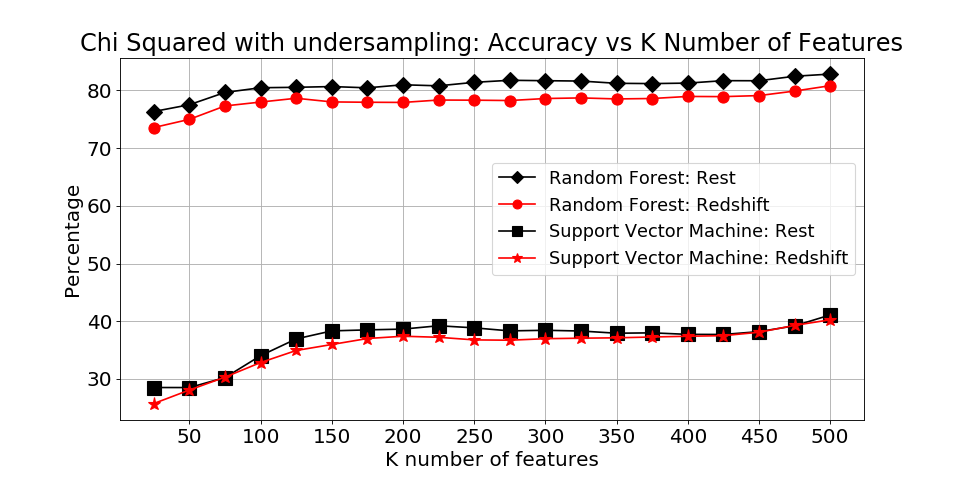
\includegraphics[width=3.5in]{Chi_Squared_Undersampled.png}
            \caption{10-Fold cross validation results for Chi Squared feature selection with undersampling for redshifted spectra and artificial rest spectra}
            \label{fig:chi-U}
        \end{figure}

	\begin{table}
\caption{10-Fold cross validation results for Chi Squared feature selection with undersampling (12,584 samples) for redshifted spectra and artificial rest spectra}
        \label{tab:chi-U}
        \resizebox{3.5in}{!}{
        \def\arraystretch{1.5}
	\begin{tabular}{|c|c|c|c|c|c|c|c|c|c|c|} \hline
\multirow{2}{*}{Classifier} & \multicolumn{10}{c|}{Accuracy (\%) for Chi Squared for K number of features} \\ 
   & 50.0 &   100.0 &   150.0 &   200.0 &   250.0 &   300.0 &   350.0 &   400.0 &   450.0 &  500.0  \\ \hline
\multicolumn{11}{|c|}{redshifted spectra} \\ \hline
RF & 76.60 & 80.81 & 80.66 & 80.88 & 80.92 & 81.64 & 81.99 & 81.79 & 82.13 & 83.59 \\ \hline
SVM & 28.33 & 33.60 & 37.64 & 37.95 & 38.73 & 39.01 & 39.02 & 38.97 & 39.13 & 40.41 \\ \hline
\multicolumn{11}{|c|}{artificial rest spectra} \\ \hline
RF & 81.81 &   86.17 &   86.03 &   86.13 &   86.72 &   86.85 &   86.82 &   86.89 &   86.92 &   88.24 \\ \hline
SVM & 29.13 &   35.69 &   38.63 &   39.13 &   39.59 &   39.82 &   40.27 &   39.87 &   39.68 &   41.27 \\ \hline
\end{tabular}}
	\end{table}

	% Chi Squared Hybrid results
        \begin{figure}
            \centering
            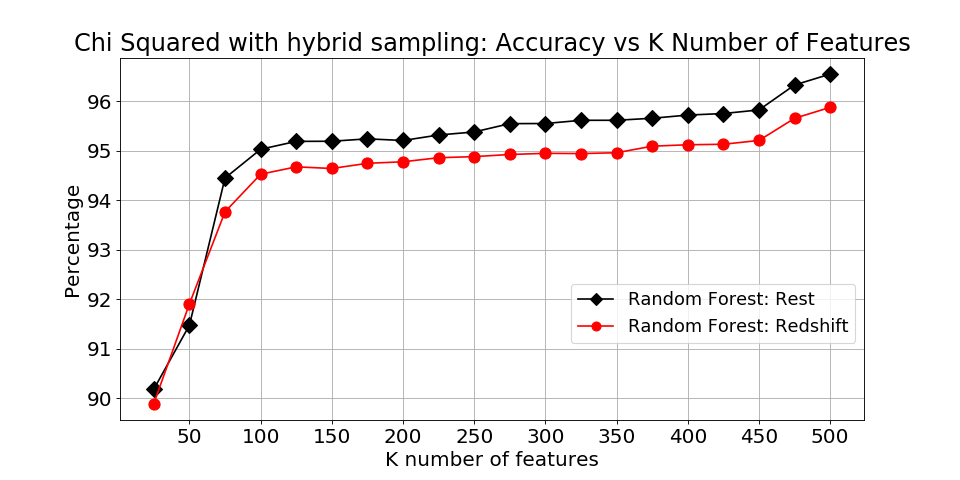
\includegraphics[width=3.5in]{Chi_Squared_Hybrid.png}
            \caption{10-Fold cross validation results for Chi Squared feature selection with hybrid sampling for redshifted spectra and artificial rest spectra spectra}
            \label{fig:chi-H}
        \end{figure}

	\begin{table}
\caption{10-Fold cross validation results for Chi Squared feature selection with hybrid sampling (367,004 samples) for redshifted spectra and artificial artificial rest spectra using Random Forest}
        \label{tab:chi-H}
        \resizebox{3.5in}{!}{
        \def\arraystretch{1.5}
	\begin{tabular}{|c|c|c|c|c|c|c|c|c|c|} \hline
\multicolumn{10}{|c|}{Accuracy (\%) for Chi Squared for K number of features} \\ 
   50.0 &   100.0 &   150.0 &   200.0 &   250.0 &   300.0 &   350.0 &   400.0 &   450.0 &  500.0  \\ \hline
\multicolumn{10}{|c|}{redshifted spectra} \\ \hline
91.24 & 95.11    & 95.25   & 95.24  & 95.46   & 95.62    & 95.65   & 95.76   & 95.90   & 96.55 \\ \hline
\multicolumn{10}{|c|}{artificial rest spectra} \\ \hline
94.34 &   97.02 &   97.03 &   97.14 &   97.31 &   97.45 &   97.43 &   97.54 &   97.65 &   98.21 \\ \hline 
\end{tabular}}
\end{table}

% ----------------------------------------------------------------------------------------------------------------------------------
	% Fisher Undersampled results
        \begin{figure}
            \centering
            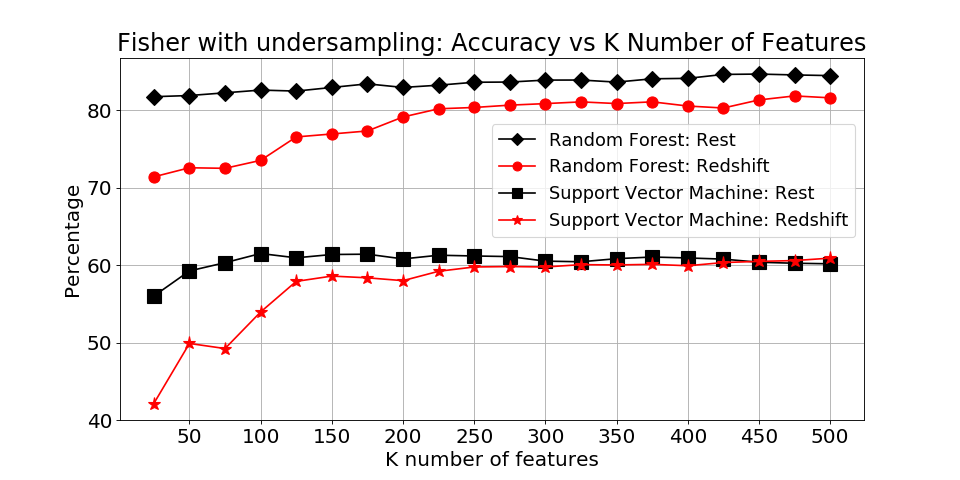
\includegraphics[width=3.5in]{Fisher_Undersampled.png}
            \caption{10-Fold cross validation results for Fisher feature selection with undersampling for redshifted spectra and artificial artificial rest spectra}
            \label{fig:fisher-U}
        \end{figure}

	\begin{table}
\caption{10-Fold Cross Validation Results for Fisher feature selection with undersampling (12,584 samples) for redshifted spectra and artificial artificial rest spectra}
        \label{tab:fisher-U}
        \resizebox{3.5in}{!}{
        \def\arraystretch{1.5}
	\begin{tabular}{|c|c|c|c|c|c|c|c|c|c|c|} \hline

\multirow{2}{*}{Classifier} & \multicolumn{10}{c|}{Accuracy (\%) for Fisher for K number of features} \\ 
   & 50.0 &   100.0 &   150.0 &   200.0 &   250.0 &   300.0 &   350.0 &   400.0 &   450.0 &  500.0  \\ \hline
\multicolumn{11}{|c|}{redshifted spectra} \\ \hline

RF & 81.177 & 82.00 & 82.79 & 83.51 & 83.45 & 83.73 & 83.26 & 83.90 & 84.52 & 84.95 \\ \hline
SVM & 60.43 & 66.51 & 65.62 & 64.83 & 64.44 & 64.48 & 65.21 & 65.33 & 64.94 & 64.66 \\ \hline
\multicolumn{11}{|c|}{artificial rest spectra} \\ \hline
RF & 83.64 &   83.46 &   85.29 &   86.29 &   86.27 &   86.19 &   86.43 &   87.16 &   87.19 &   87.40 \\ \hline
SVM & 55.63 &   56.06 &   57.29 &   58.73 &   61.02 &   62.23 &   62.59 &   63.21 &   63.63 &   63.81 \\ \hline
\end{tabular}}
	\end{table}

	% Fisher Hybrid results
        \begin{figure}
            \centering
            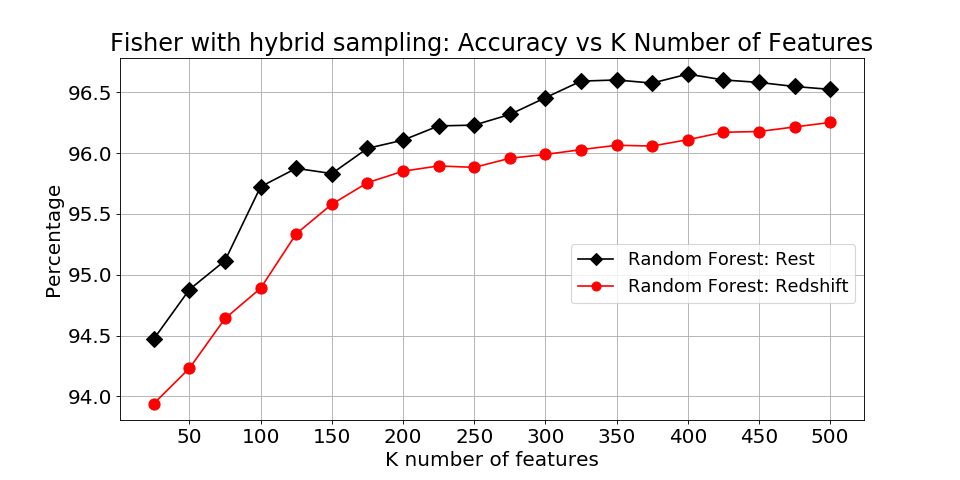
\includegraphics[width=3.5in]{Fisher_Hybrid.png}
            \caption{10-Fold cross validation results for Fisher feature selection with hybrid sampling for redshifted spectra and artificial artificial rest spectra}
            \label{fig:fisher-H}
        \end{figure}

	\begin{table}
\caption{10-Fold cross validation results for Fisher feature selection with hybrid sampling (367,004 samples) for redshifted spectra and artificial artificial rest spectra using Random Forest}
        \label{tab:fisher-H}
        \resizebox{3.5in}{!}{
        \def\arraystretch{1.5}
	\begin{tabular}{|c|c|c|c|c|c|c|c|c|c|} \hline

\multicolumn{10}{|c|}{Accuracy (\%) for Fisher for K number of features} \\ 
   50.0 &   100.0 &   150.0 &   200.0 &   250.0 &   300.0 &   350.0 &   400.0 &   450.0 &  500.0  \\ \hline
\multicolumn{10}{|c|}{redshifted spectra} \\ \hline

94.65 & 95.89 & 96.22 & 96.38 & 96.49 & 96.59 & 96.62 & 96.74 & 96.79 & 96.87 \\ \hline
\multicolumn{10}{|c|}{artificial rest spectra} \\ \hline
96.30 &   97.22 &   97.51 &   97.59 &   97.58 &   97.44 &   97.37 &   97.36 &   97.32 &   97.32 \\ \hline
\end{tabular}}
	\end{table}

	% Fisher results
        \begin{figure}
            \centering
            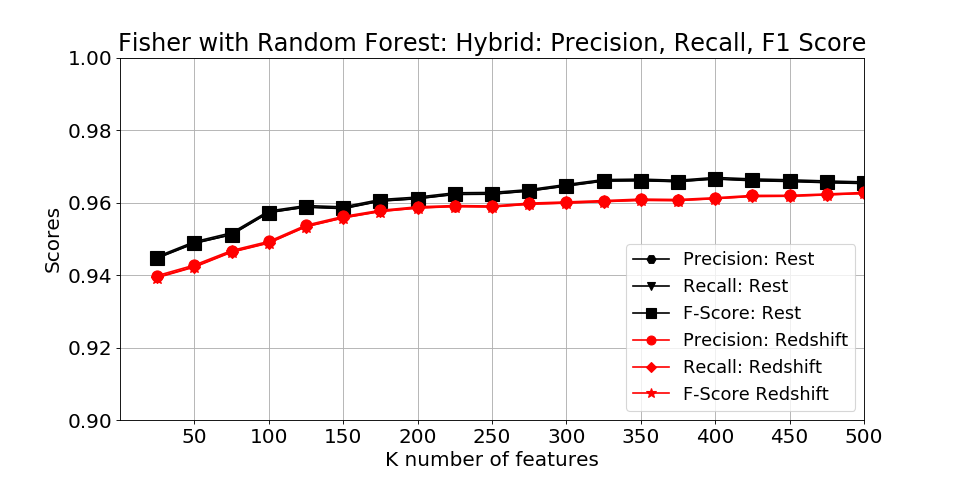
\includegraphics[width=3.5in]{Results3.png}
            \caption{Average results of five experiments for Fisher feature selection for random forest}
            \label{fig:results}
        \end{figure}

	\begin{table}
	\caption{Precision, Recall, and F1 Score for Fisher feature selection with Hybrid for Random Forest}
        \label{tab:results1}
        \resizebox{3.5in}{!}{
        \def\arraystretch{1.5}
	\begin{tabular}{|c|c|c|c|c|c|c|c|c|c|c|}
	\hline

\multirow{2}{*}{} & \multicolumn{10}{c|}{Results for Fisher + Random Forest for K number of features} \\ 
   & 50.0 &   100.0 &   150.0 &   200.0 &   250.0 &   300.0 &   350.0 &   400.0 &   450.0 &  500.0  \\ \hline
\multicolumn{11}{|c|}{redshifted spectra} \\ \hline
Precision & 0.9474 &  0.9593 &  0.9626 &  0.9642 &  0.9652 &  0.9662 &  0.9665 &  0.9677 &  0.9682 &  0.9690 \\ \hline
Recall & 0.9465 &  0.9589 &  0.9622 &  0.9638 &  0.9649 &  0.9659 &  0.9662 &  0.9674 &  0.9679 &  0.9687 \\ \hline
F1 Score & 0.9467 &  0.9589 &  0.9622 &  0.9639 &  0.9649 &  0.9659 &  0.9662 &  0.9674 &  0.9680 &  0.9687 \\ \hline
\multicolumn{11}{|c|}{artificial rest spectra} \\ \hline
Precision & 0.9634 &  0.9724 &  0.9753 &  0.9761 &  0.9760 &  0.9746 &  0.9740 &  0.9739 &  0.9735 &  0.9735 \\ \hline
Recall & 0.9630 &  0.9722 &  0.9751 &  0.9759 &  0.9758 &  0.9744 &  0.9737 &  0.9736 &  0.9732 &  0.9732 \\ \hline
F1 Score &  0.9630 &  0.9722 &  0.9751 &  0.9759 &  0.9758 &  0.9744 &  0.9738 &  0.9736 &  0.9732 &  0.9732 \\ \hline
	\end{tabular}}
	\end{table}

%------------------------------------------------------------------------------
\newcolumntype{L}{>{\centering\arraybackslash}m{1.7cm}}
% Execution Times
	\begin{table}
	\caption{Execution time for hybrid sampling for random forest with artificial rest spectra}
        \label{tab:time}
	\LARGE
        \resizebox{3.5in}{!}{
        \def\arraystretch{1.5}
	\begin{tabular}{|c|L|L|L|L|L|L|L|L|L|L|}
	\hline
\multirow{2}{*}{} & \multicolumn{10}{c|}{Execution times (Seconds) for K number of features} \\ 
   & 50.0 &   100.0 &   150.0 &   200.0 &   250.0 &   300.0 &   350.0 &   400.0 &   450.0 &  500.0  \\ \hline
\multicolumn{11}{|c|}{Fisher + artificial rest spectra} \\ \hline
\def\arraystretch{1.1} \begin{tabular}{c} Feature\\Selection\end{tabular} &  7.94 $\times$ 10$^5$ & 7.94 $\times$ 10$^5$ & 7.94 $\times$ 10$^5$ & 7.94 $\times$ 10$^5$ & 7.94 $\times$ 10$^5$ & 7.94 $\times$ 10$^5$ & 7.94 $\times$ 10$^5$ & 7.94 $\times$ 10$^5$ & 7.94 $\times$ 10$^5$ & 7.94 $\times$ 10$^5$ \\ \hline
   Train &  39.83 &     55.49 &     66.23 &     76.77 &     82.10 &     93.07 &     99.46 &    110.21 &    115.85 &    121.24 \\\hline
   Test &  0.65 &      0.58 &      0.61 &      0.62 &      0.63 &      0.68 &      0.69 &      0.70 &      0.75 &      0.79 \\ \hline

\multicolumn{11}{|c|}{Chi Squared + artificial rest spectra} \\ \hline
\def\arraystretch{1.1} \begin{tabular}{c} Feature\\Selection\end{tabular} & 6.84 &    7.98 &    9.12 &   10.41 &   11.21 &   12.40 &   13.24 &   14.72 &   16.13 &   17.48 \\ \hline
   Train &  37.11 &   50.08 &   60.03 &   69.79 &   75.07 &   84.80 &   90.28 &  100.28 &  105.45 &  109.06 \\ \hline
   Test &  0.57 &    0.55 &    0.57 &    0.60 &    0.62 &    0.64 &    0.68 &    0.70 &    0.73 &    0.74 \\ \hline
	\end{tabular}}
	\end{table}


% ============================================================================================================
	\subsection{Implementation}\label{sec:imp}

	The experiments presented in this paper are implemented using Python and scikit-learn \cite{scikit-learn}. Due to the size of the imbalanced raw dataset (35.4 GB for artificial rest spectra and 35.4 GB for redshifted spectra), the Python NumPy memmap \cite{numpy, memmap} module was utilized to read very large arrays from storage rather than RAM. We run our test on an IBM S822LC cluster with IBM POWER 8 nodes, NVLink and NVidia Tesla P100 GPUs \cite{turing}.

	\hlorange{RF and SVM are implemented with scikit-learn with default parameters} \cite{scikit-learn}. \hlorange{SVM is implemented using a Gaussian kernel}. Precision, recall, and F1 score are computed using functions implemented by the scikit-learn sklearn.metrics package \cite{scikit-learn}. The Chi Squared feature selection algorithm is implemented using scikit-learn \cite{scikit-learn}. The Fisher feature selection algorithm is implemented using scikit-feature \cite{reliefF}.
% ============================================================================================================
	\subsection{Discussion}\label{sec:disc}

	Figs. \ref{fig:chi-U}, \ref{fig:chi-H}, \ref{fig:fisher-U} and \ref{fig:fisher-H} show that classification using the redshift spectra has essentially the same accuracy as the artificial rest spectra, despite the fact that redshift has introduced problematic data into the feature matrix. Figs. \ref{fig:chi-U} and  \ref{fig:fisher-U} also demonstrate that RF is the best classifier for both redshifted spectra and artificial rest spectra. 

	Tables \ref{tab:chi-U} and \ref{tab:fisher-U} show that the Fisher method performs better than Chi Squared method for both redshifted spectra and artificial rest spectra when using the RF classifier. From Tables \ref{tab:chi-H} and \ref{tab:fisher-H} we observe that with the Fisher feature selection method we obtain roughly a one percent higher accuracy than with the Chi Squared method. However, Table \ref{tab:time} demonstrates that Chi Squared has a significantly shorter execution times than Fisher. 

	Tables \ref{tab:chi-U}, \ref{tab:chi-H}, \ref{tab:fisher-U}, and \ref{tab:fisher-H} demonstrate that hybrid sampling outperforms undersampling. Tables \ref{tab:chi-U}, \ref{tab:chi-H}, \ref{tab:fisher-U}, and \ref{tab:fisher-H} show that accuracy increases with more samples. Supplementing SDSS data run 14 with samples from SDSS data run 12, 13, and 15 may improve accuracy.

	Fig. \ref{fig:results} shows that the precision, recall, and F1 scores for redshifted spectra are lower than for artificial rest spectra. However, Table \ref{tab:results1} show that the precision for redshifted spectra is only lower by 0.0045, recall is only lower by 0.0045 and the F1 score is lower by 0.0045 (for 500 features).  

	For redshifted spectra, we achieved an accuracy of 96.87\% using the Fisher feature selection with hybrid sampling using the RF classifier applied to 500 selected flux measurements. Using the same work flow, we obtained 97.32\% accuracy for artificial rest spectra. These results are superior by more than three percent than the ones achieved by Xing \textit{et al.} \cite{Xing}, since they reported 93.26\% accuracy using wavelet reduction and SVMs for SDSS spectra. 
	
Bolton \textit{et al.} used Chi Squared minimization to determine the redshift and classification of SDSS spectra of galaxies, quasars, and stars \cite{Bolton}. They applied the Least Squares minimization to compare each spectrum to a full range of templates that span through galaxies, quasars, and stars. Our approach takes considerably fewer steps than the one in \cite{Bolton} and produces excellent results. 

%	Fig \ref{fig:time} shows that the execution times for both redshifted spectra and artificial rest spectra are approximately the same for Chi Squared and Random Forest. Table \ref{tab:time} shows that the Random Forest testing time is 1.27 seconds and 1.24 seconds for artificial rest spectra and redshifted spectra respectively. The time for feature selection for redshifted spectra for the best 240 flux measurements is 1,439.89 seconds, as seen in Table \ref{tab:time}. 

The execution times and the obtained accuracy demonstrate that, for a real application of this work, the automated classification of redshifted stellar spectra not only achieves a high accuracy but is also fast. 

%It is an important reminder that the SDSS dataset that is used for this paper do not contain the M-K luminosity classes. 
% ============================================================================================================
\section{Conclusions}\label{sec:conclusion}

According to our results, accurate stellar classifications can be obtained using a combination of domain specific data pre-processing, feature selection  and classification techniques. Compared to previous work of other authors, we have two interesting conclusions:

\begin{enumerate}
	\item Redshift corrections are not necessary to obtain this high level of accuracy.
	\item Aside from wavelength fitting and flux scaling, any additional spectrum pre-processing after the processes presented by Dawson \textit{et al.} \cite{Dawson} and Stoughton \textit{et al.} \cite{Stoughton} is unnecessary. 
\end{enumerate}

Therefore, when a star can be accurately classified prior to redshift correction, many stellar properties can be easily attained without the complex data transformations and statistical analyzes used by other authors. 

%"Saving this for the thesis" As a result of this claim, if a stellar spectrum can be classified then information that would normally involve complex data transformations and analysis become easily available, such as emission and absorption lines, redshift values, radial velocities, effective surface temperature, and more. \todo[inline]{use this in conclusions?}

Even though the feature matrix for redshifted stellar spectra produces an undesired feature matrix because of flux discrepancies, high accuracy was still achieved. This can be accounted for by redshift values for stars being small and a large sample of redshift values to train the classifier.

%Through the process of building the feature matrix for redshifted stellar spectra they produce an undesired feature matrix, explained in more detail in Section \ref{sec:feature} and seen in Table \ref{tab:example}. We claim that even though this feature matrix has discrepancies, high accuracy can still be achieved due to the redshift values for stars being small. The results support this claim. \todo[inline]{use this in conclusions?}

%	In this paper, we discussed how we processed the data, how we construct the feature matrix, and how we handled missing values. We then compared Chi Squared feature selection for Random Forest, Support Vector Machine, and Naive Bayes classifier algorithms. We then compared redshifted spectra to artificial rest spectra. Based on the results of these experiments, even though redshift causes discrepancies in the feature matrix, excellent results can still be attained. Based on these results, we propose that using feature selection and classifier algorithms before redshift correction is a viable approach to stellar classification and that with future work, stellar properties can be easily attained once the stellar class is known. 


\IEEEtriggeratref{27}

\raggedright
\bibliographystyle{IEEEtran}
\bibliography{ref}

\end{document}